\graphicspath{{images_low_res/}}
\section{Approach}
\label{sec:approach}

\subsection{Develop an Initial Model}
\label{sec:initial_model}



Figure~\ref{fig:simple_model} shows a schematic of our initial approach to modelling (nutrient dependent growth with nutrient and signal diffusion).
Each culture on the agar is given a label, \(i\), and has three variables associated with it: one observed variable, \(C_{i}\), the amount of cells in the culture at location \(i\), and two hidden variables, \(N_{i}\), the amount of nutrients at location \(i\), and \(S_{i}\), the amount of signal molecule location \(i\).
Cultures in QFA and SGA agars are arranged in a square array, each culture having eight neighbours with which they could conceivably interact with directly. Initially, we will model diffusion between only the four closest neighbours, in the vertical and horizontal directions (darker blue circles in Figure~\ref{fig:simple_model}).
We will describe nutrient dependent growth at each location using mass action kinetics and the following reaction equation:
\begin{equation}
  \label{eq:1}
  C + N \xrightarrow[]{r_{i}} 2C,\\
\end{equation}
where \(r_{i}\) is the rate constant of conversion at location \(i\).
As a first approach, assuming that the number of cells is continuous, we will incorporate the effect of signal molecules on growth and the diffusion of both nutrient and signal molecules using the following ODEs:
\begin{subequations}
  \label{eq:2}
  \begin{align}
    \frac{dC_{i}}{dt}& = r_{i}N_{i}C_{i} - \beta S_{i},\\
    \frac{dN_{i}}{dt}& = - r_{i}N_{i}C_{i} - k_{n}\sum_{j}(N_{i} - N_{j}),\\
    \frac{dS_{i}}{dt}& = \alpha C_{i} - k_{s}\sum_{j}(S_{i} - S_{j}),
  \end{align}
\end{subequations}
where, \(j\) indicates the closest neighbours, \(k_{n}\) and \(k_{s}\) are nutrient and signal diffusion constants, \(\alpha\) is the rate of secretion of signal, and \(\beta\) is a constant for the effect of signal on culture population. Alternative models for signalling effect could be used; initially, we have chosen to use the simplest. Setting diffusion constants to zero reduces \ref{eq:2} to the independence model. We may also study the effects of signalling and competition for nutrients separately by setting other parameters to zero. If necessary, diagonal neighbours could be incorporated into this model by adding or scaling diffusion constants. In section~\ref{sec:dev-mod-further}, we discuss the possibility of using finer-grain spatially-discretised or continuous models of diffusion.
% \begin{equation}
%   \label{eq:3}
%   \frac{dC_{i}}{dt}& = r_{i}N_{i}C_{i}(1 - \frac{S_{i}}{S_{crit}})
% \end{equation}

\begin{Figure}
  \centering
  \includegraphics[width=\linewidth]{square_array}
  \captionof{figure}{Schematic of simple modelling approach.}
  \label{fig:simple_model}
\end{Figure}


Models will be written in SBML (ref), using SBML shorthand (ref), so that they may eventually be published in the BioModels database (ref) and reused by the scientific community. This will require conformation to the minimum information standard MIRIAM (ref). (Simulation experiments should also conform to MIASE (ref).) We will write code for the rest of the project in Python as this has several advantages: it is used widely by the scientific community, has libraries which will be of use to us, and related tools such as Colonyzer (ref) are already written in Python. To interface SBML models with Python we will use the libSBMLO library \citep{Bornstein2008}. ODEs will be solved using odeint from the SciPy library \citep{SciPy}. We will use git as version control and use GitHub as a remote repository to allow collaboration and so that tools may eventually be released publicly.

It is anticipated that solving sets of ODEs for typically 384 cultures in QFA and 1536 cultures in SGA will be take a long time. Therefore, while testing, we will simulate smaller sets of artificial data from the ODE models and attempt to fit these. We will also incorporate unittesting into the development to try to ensure that the code will still work when scaled up to larger arrays used in experiments.

\subsection{Analyse Experimental Data}
\label{sec:analyse-data}
We have access to unpublished QFA and SGA data for the model organism \textit{S. Cerevisiae}. Some data (Figure~\ref{fig:gaps}), with uncultured gaps, is specifically designed for the study of competition.


\subsection{Develop Model Further}
\label{sec:dev-mod-further}

\begin{Figure}
  \centering
  \includegraphics[width=\linewidth]{square_array_grid}
  \captionof{figure}{Schematic of a spatially-discretized two-dimensional model.}
\end{Figure}

\begin{Figure}
  \centering
  \includegraphics[width=\linewidth]{height_dep_miniqfa_delta_z}
  \captionof{figure}{Schematics of diffusion across agar height.}
\end{Figure}
% Could model movement of vertical or movement across it.
\subsection{Compare Experimental Designs}
\label{sec:comp-exper-designs}


\begin{Figure}
  \centering
  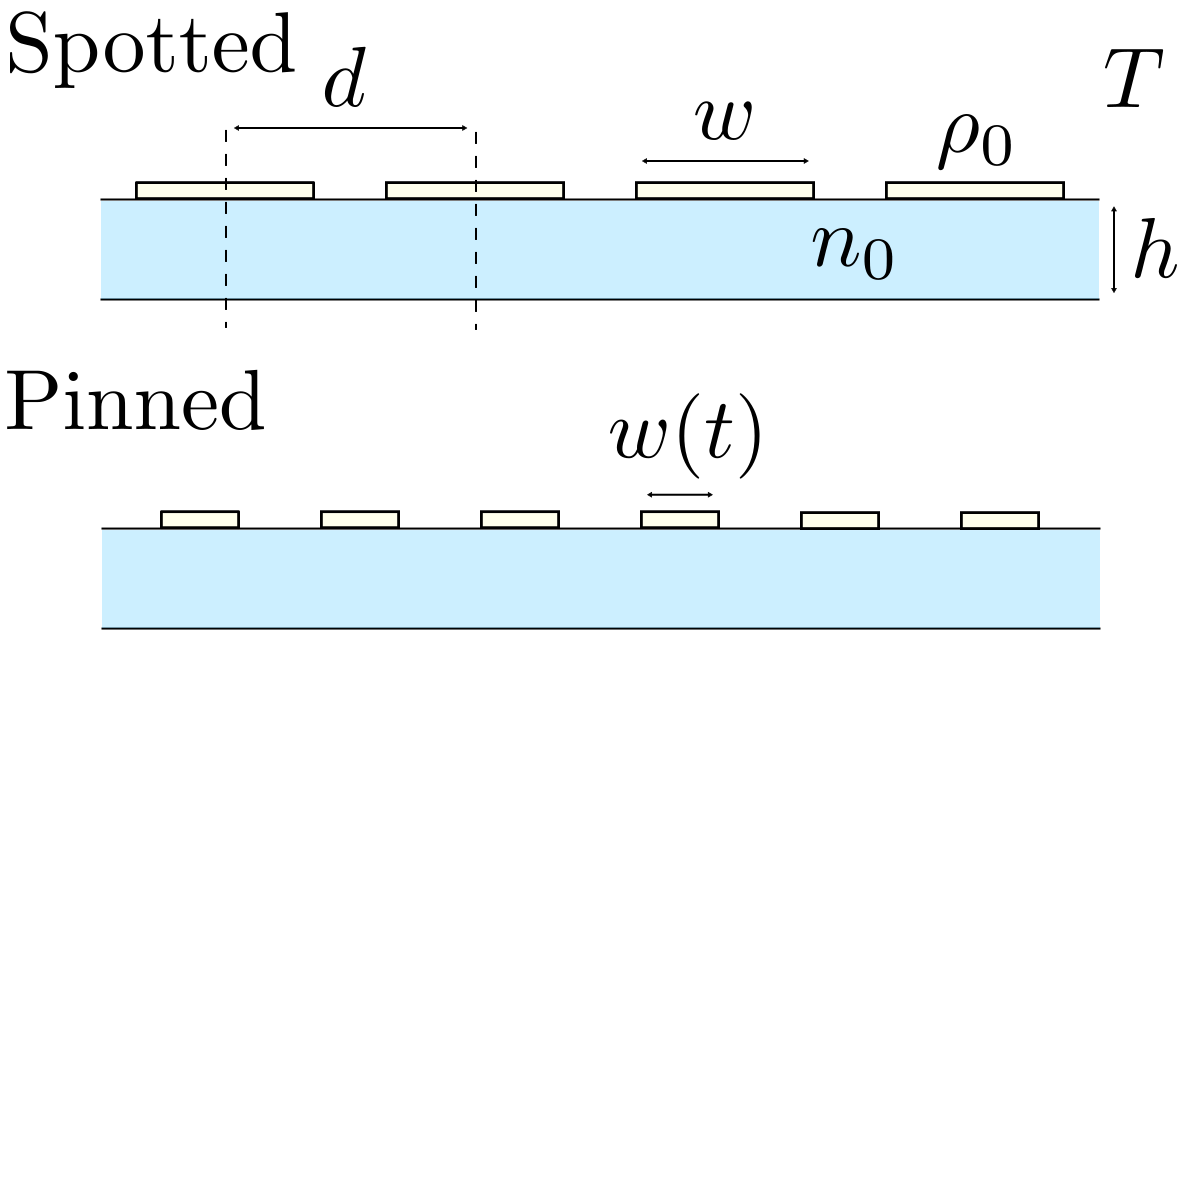
\includegraphics[width=\linewidth]{qfa_v_sga_vars}
  \captionof{figure}{QFA and SGA agars.}
\end{Figure}



\begin{Figure}
  \centering
  \includegraphics[width=\linewidth]{gaps}
  \captionof{figure}{An agar, with locations left empty (``gaps''), designed to exhibit effects of competition and signalling.}
\end{Figure}

\begin{Figure}
  \centering
  \includegraphics[width=\linewidth]{stripes}
  \captionof{figure}{A miniQFA agar in which lines of locations (``stripes'') are left uncultured. We can use a similar experimental setup, with uniform cultures in one dimension, to study diffusion across agar height in only two dimensions.}
\end{Figure}

\subsection{Package and Distribute}
\label{sec:package-distribute}


%%% Local Variables:
%%% mode: latex
%%% TeX-master: "proposal"
%%% End:
